\documentclass[10pt, final]{beamer}

\mode<presentation>
{
  \usetheme{mpe}
}
\graphicspath{{figures/}{../../../Assets/SharedFigures/}} % local figures + shared

\usepackage{ragged2e}
\usepackage{lipsum}
\usepackage{subcaption}
\usepackage{xspace}
\captionsetup{compatibility=false}

\usepackage{graphicx}
\usepackage{tikz}

\usepackage{amsmath,amssymb}
\usepackage[english]{babel}
\usepackage[latin1]{inputenc}
%\usepackage{tristan-presentation}
\usepackage[orientation=landscape,size=a0,scale=0.95,debug]{beamerposter} 

\title[I like to make posters]{A novel scaling early warning indicator\\ and its application to tropical cyclones}

\author[T]{Joshua Prettyman}

\institute[SMS]{University of Reading\\ National Physical Laboratory}

\date{\today}

\newcommand{\pd}[2]{\ensuremath{\partial_{#1}{#2}}\xspace}
\renewcommand{\div}{\operatorname{div}}
\renewcommand{\vec}[1]{{\bf #1}}
\providecommand{\figwidth}{\textwidth}
\newcommand{\figscale}{1.2}

%\setlength{\leftmargini}{20pt}

\captionsetup[figure]{format=hang,indention=-60pt,margin=50pt}

\begin{document}



\begin{frame}{} 
  \begin{columns}[T]
    \begin{column}{0.25\textwidth}
    		\begin{block}{Introduction}
    		
    		Many physical systems are governed by dynamics that permit more than one state, such as the glacial/interglacial cycle of our climate. Moreover, a bifurcation in the dynamics may change the number of permitted states. \\
    		\vspace{0.5cm}
    		A dramatic and relatively sudden shift from one state to another is known as a tipping point. Hopefully the time series from a measurement of the system will reveal the tipping point. \\
    		\vspace{0.5cm}
	
		It is usual to think about a tipping point as the point in time at which a stable mode collapses - a steady state, a stable orbit, a limit cycle or a potential well. These modes which are approaching collapse we refer to a critical modes. \\
    		\vspace{0.5cm}		
		When measuring any property of a time series with a time lag, we may consider how the property scales with time and infer an estimate of the decay rate - the rate at which the mode is decaying towards the tipping point. \\
    		\vspace{0.5cm}			
	
    		This PhD project aims to develop a multi-purpose prediction tool for tipping points in physical systems. Several techniques are used to analyse time series for Early Warning Signals.	 These techniques are also applied to toy models in order to understand their limitations. This poster is adapted from the recent paper by Prettyman et al. [8].
    		\end{block}  
    			
    
    

    
    \begin{block}{A Simple Example of a Tipping Point: Pitchfork Bifurcation}
    \begin{columns}[T]
    		\begin{column}{0.5\textwidth}
    Equation (\ref{eqn1}) describes a stochastic dynamical system $z(t)$ in the form of a potential function with added noise $\eta_t$. The shape of the potential function changes as $t$ increases (see figure, right), removing the stable mode at $z=0$ and creating a double well potential.
    \vspace{0.3cm}
\begin{align}
\dot{z}(t) & = -\frac{\partial}{\partial z}(z^4 + \left(3-\frac{t}{200}\right)z^2) + \eta_t
\label{eqn1}
\end{align}
		\end{column}
		\begin{column}{0.4\textwidth}
\begin{figure}

\includegraphics[width = \textwidth]{changing_potential.png} \caption{The shape of the potential at various times. Note the bifurcation at $t=600$.}
\end{figure}
		
		\end{column}
	\end{columns}
	\vspace{1cm}
\begin{figure}

\includegraphics[]{Fig3_colour.png} \caption{100 model runs (a) with the 100-point indicators ACF(1), DFA and PS (b,c,d resp.).\\ Figures show the mean indicator value with error bars of one standard deviation.}
\end{figure}
    			It is proposed that a tipping point visible in a time series will be anticipated by a rise in the series' autocorrelation [1,2]. We calculate the ACF(1), DFA and PS scaling indicators and note the similar behaviour, although the PS indicator has a significantly larger variance. This pitchfork bifurcation model is chosen as a testbed for the novel PS indicator.
    			\end{block}
    		\end{column}
    		
    		%*********************************************
    		%*********************************************
    		%*** COLUMN 2 - THE BIG MIDDLE ONE -2222222222
    		%*** 22222222222222222222222222222222222222222
    		
    		\begin{column}{0.47\textwidth}
    			
    			\begin{block}{A Novel scaling indicator - based on the power spectrum}
    			
    			\begin{columns}[T]
    			\begin{column}{0.02\textwidth}
			\end{column}

    			\begin{column}{0.53\textwidth}
    			
    			\begin{figure}
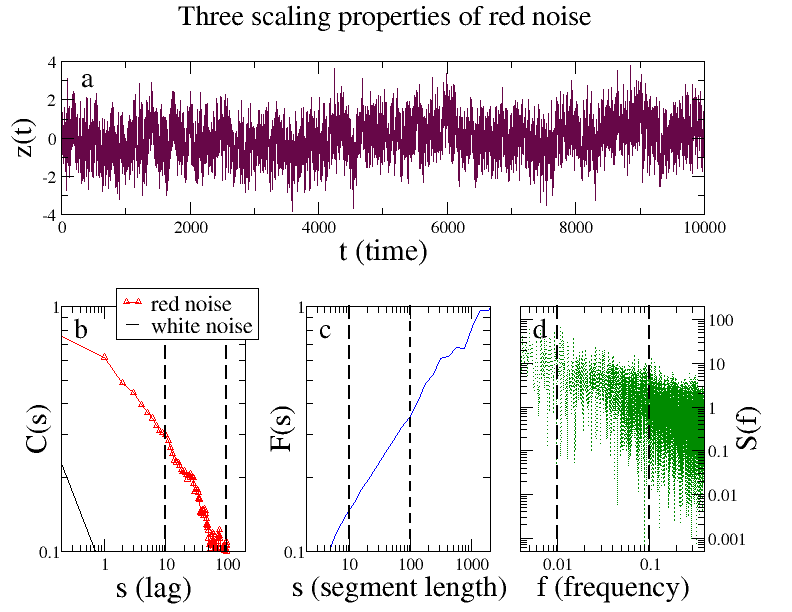
\includegraphics[width = 0.9\textwidth]{Fig1_colour.png}\caption{The three scaling exponents are applied to red noise (panel a). }
\end{figure}

Scaling properties of time series can be measured using three techniques. In the figure above we demonstrate the relationship between these scaling exponents: the autocorrelation function (ACF), detrended fluctuation analysis (DFA) and the power spectrum. \\

The first two exponents have previously been used as Early Warning Signals for tipping points. We propose also using the third option, the power spectrum scaling exponent ($\beta$). Analytically, the three scaling exponents have the linear relationship:\begin{equation} \alpha = \frac{1+\beta}{2} = 1 - \frac{\gamma}{2}. \label{analytic_relationship}
\end{equation}



			\end{column}
			\begin{column}{0.03\textwidth}
			\end{column}


			\begin{column}{0.41\textwidth}

\begin{figure}
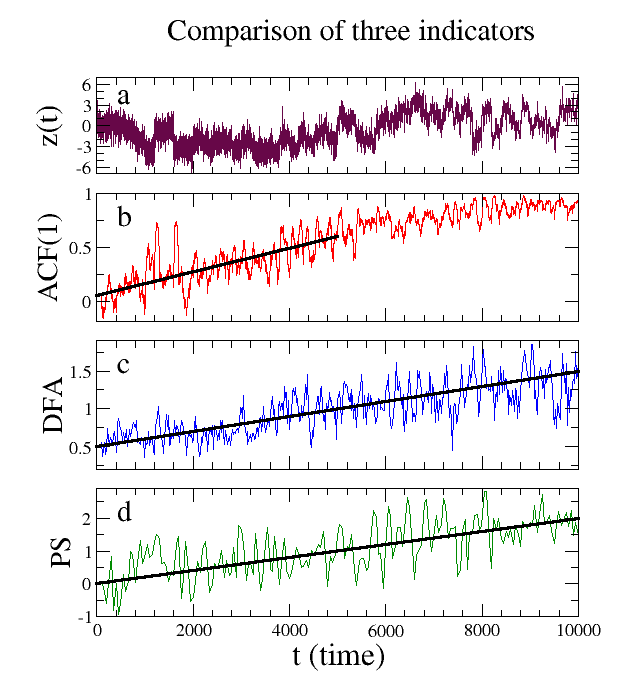
\includegraphics[width = 0.9\textwidth]{Fig2_colour.png} \caption{The three indicators are applied to an artificial time series (panel a) with increasing PS exponent.}
\end{figure}
By calculating in a sliding window we can then see the change in the exponent value over time, and so use the exponent as an EWS indicator.\\

In the figure above we have applied our three indicators to a time series constructed such that the PS indicator increases from zero to two. We are able to see that the three indicators behave similarly. 


			\end{column}
			\begin{column}{0.02\textwidth}
			\end{column}
			\end{columns}
    			    			
    			
    			\end{block}
   
   				
   			\begin{block}{Application to tropical cyclones}
   			
   			\begin{columns}
   			\begin{column}{0.02\textwidth}
			\end{column}
			\begin{column}{0.41\textwidth}
			\begin{figure}

\includegraphics[width = \textwidth]{fig4_colour.png} \caption{The three indicators (panels b,c,d) are applied to pressure data close to the landfall of 14 tropical cyclones (panel a).}
			\end{figure}
			\end{column}
			\begin{column}{0.02\textwidth}
			\end{column}
			\begin{column}{0.25\textwidth}
			We now apply the PS-indicator to data from a real geophysical system: sea-level pressure data from close to the landfall locations of 14 tropical cyclones. The 14 cyclones were selected for being ranked category 4 or 5 at the time of landfall. \\
			\vspace{0.5cm}

The tropical cyclone data does not appear to contain a bifurcation in the same sense as the pitchfork bifurcation, however, there is a tipping point in the sense that the pressure drops suddenly when the cyclone passes over, and this most likely affects the dynamics, providing a detectable EWS. The event is not analogous to the bifurcation in the pitchfork example, but is convenient to use for the purpose of comparison.\\
			\vspace{0.5cm}

We apply the indicator in a sliding window of 100 points to all 14 time series and plot the mean with error bars of one standard deviation. Again, we apply the ACF(1)-, DFA- and the new PS-indicator (panels (b,c,d)). The ACF(1)- indicator, in this case, does not appear to provide a clear EWS, whereas the PS-indicator does show an increasing trend starting at around 50 hours before the minimum pressure.
			
			
			\end{column}
			\begin{column}{0.02\textwidth}
			\end{column}
			\begin{column}{0.25\textwidth}
			
			\begin{figure}
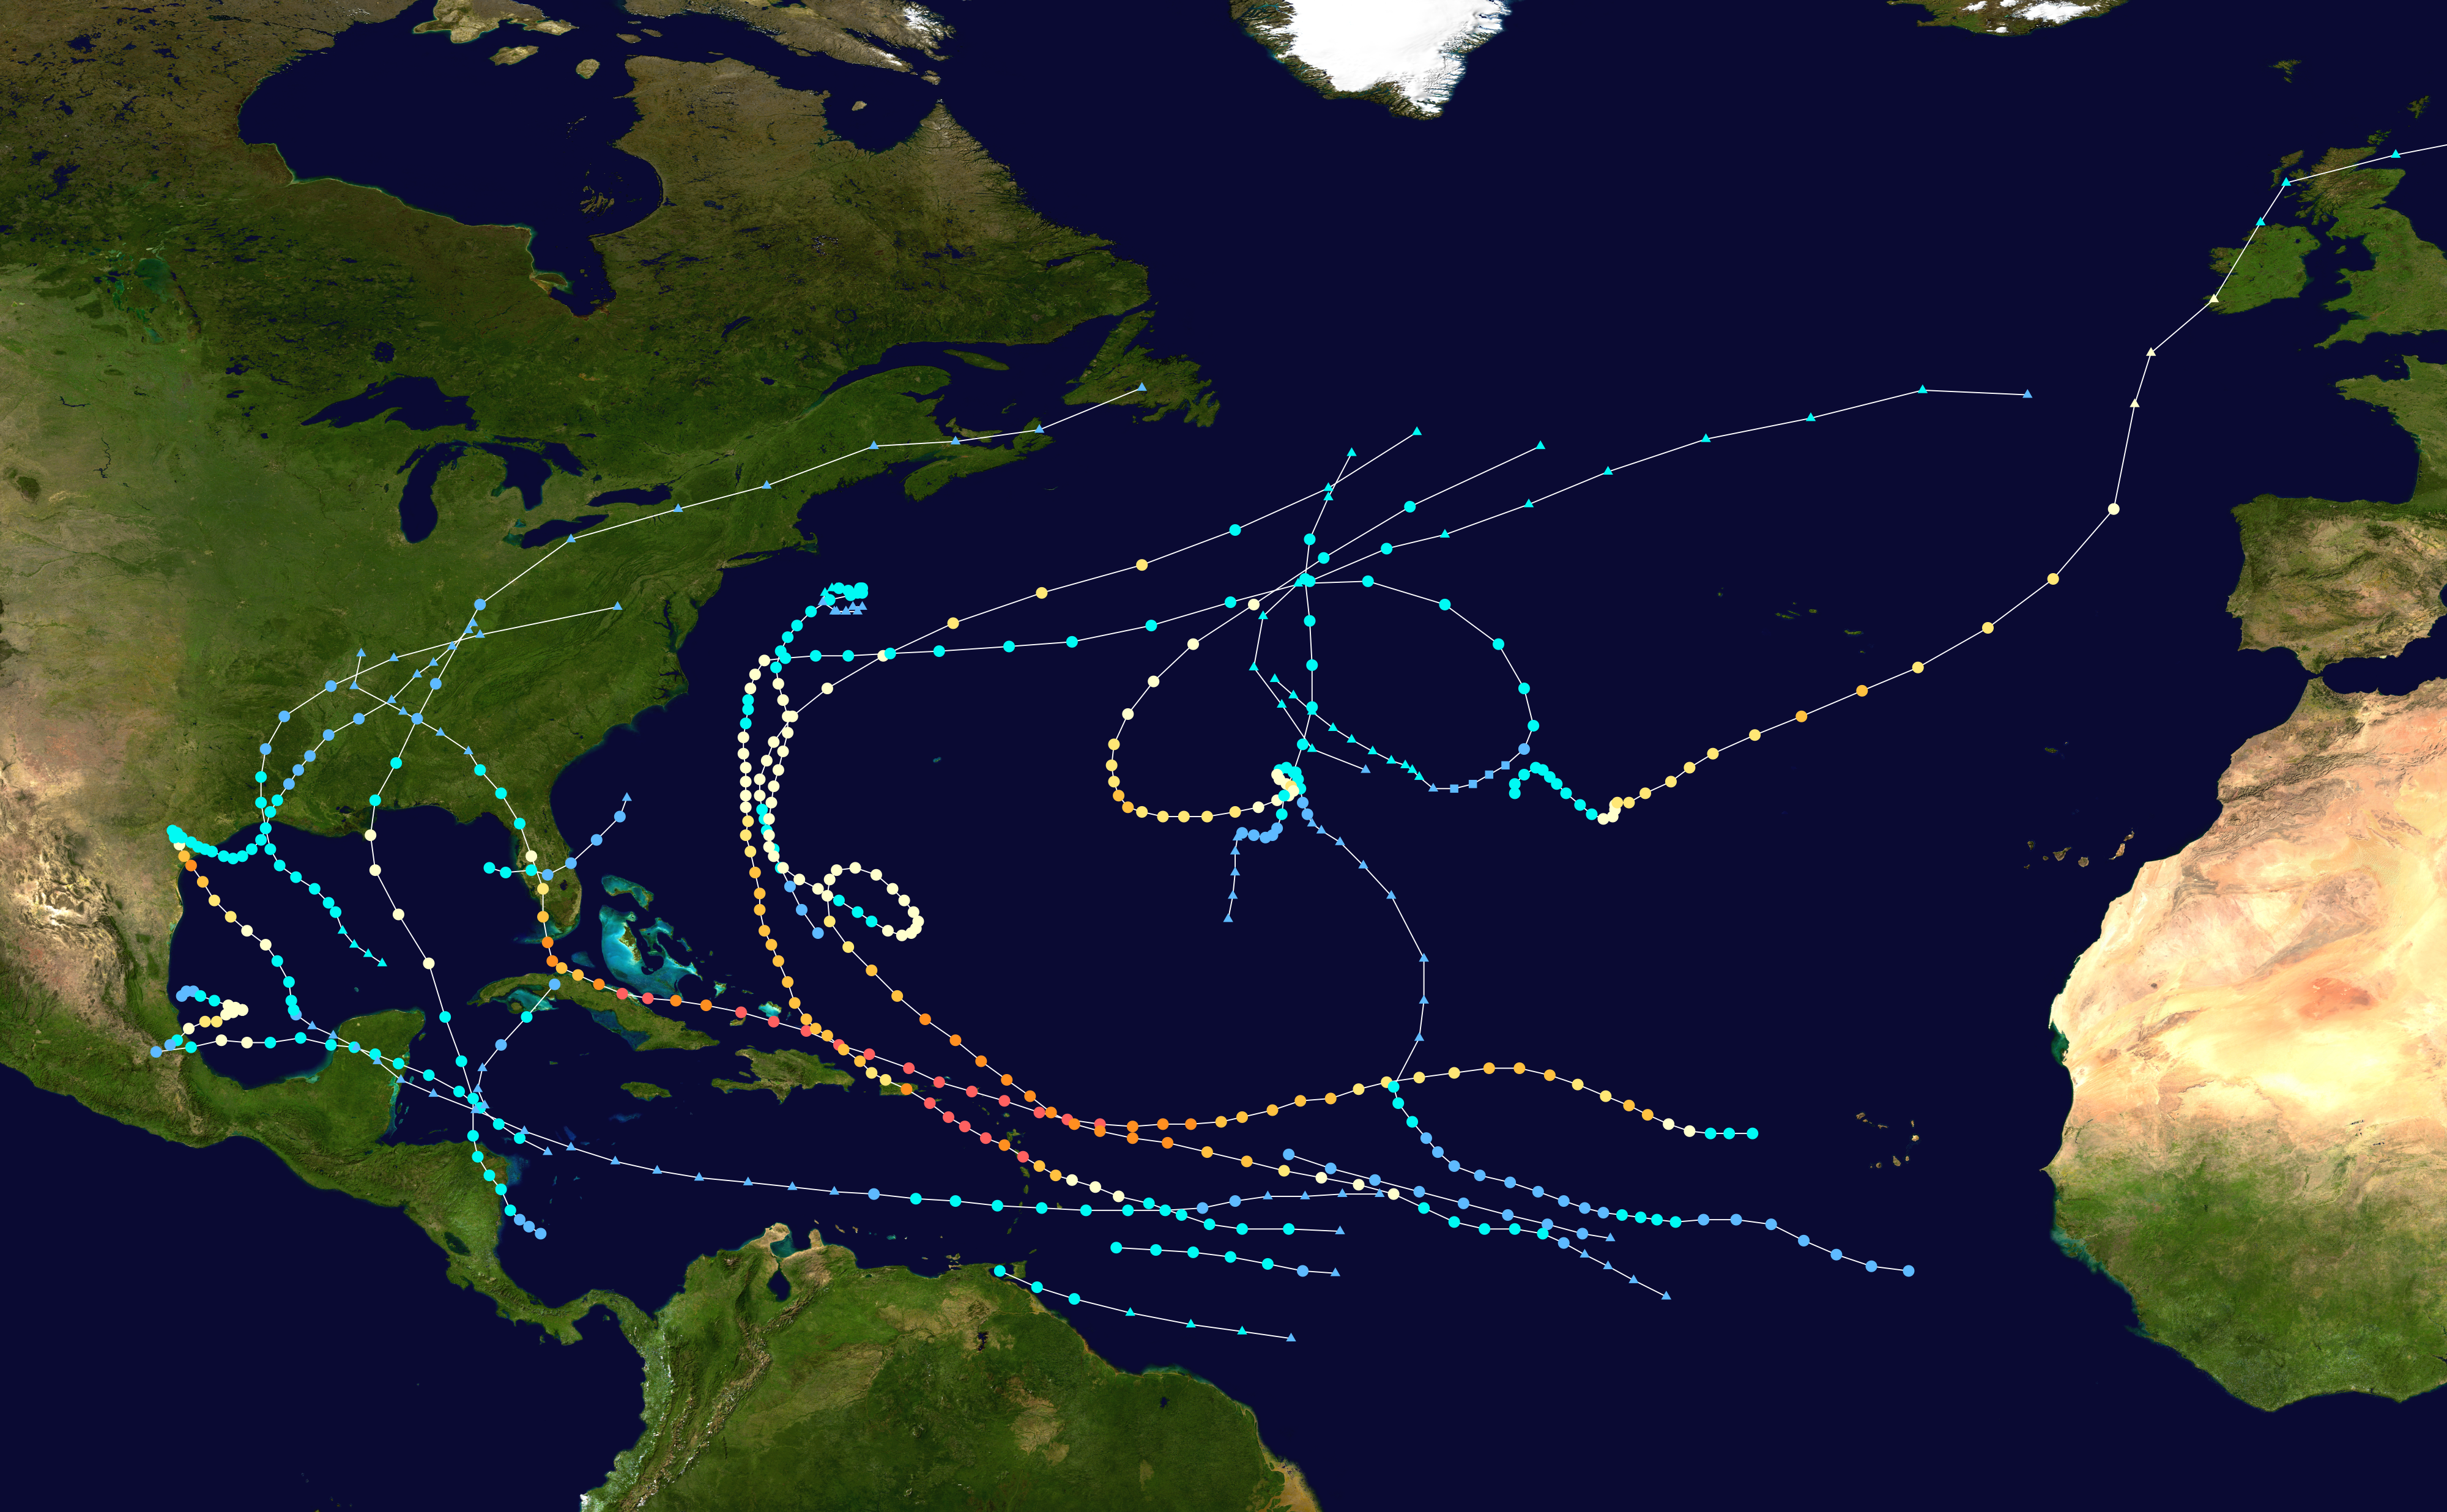
\includegraphics[width = \textwidth]{hurricanes2017.png} \caption{Storm tracks from the 2017 Atlantic hurricane season [wikimedia]}
\end{figure}

			We have thus applied the novel PS- indicator to a simple model system, and real geophysical data. The PS-indicator behaves similarly to the previously used indicators applied to the model data. When applied to the cyclone data, the other indicators do not appear to provide an EWS, but the PS-indicator clearly does begin to rise around 50 hours before the lowest pressure, about the same point that the decreasing trend becomes visible, suggesting that it can provide an EWS.\\
			\vspace{0.5cm}

The approaching cyclone is chosen as an example of a system which has not previously been studied using tipping-point EWS methods, and for which the dynamics of the system are unknown, to facilitate further investigation of this technique.
			
			\end{column}
			\begin{column}{0.02\textwidth}
			\end{column}
   			
   			
   			
   			
   			
			\end{columns}
   			\end{block}
   			
   			
   			
   			
    		\end{column}
    		 	
		%*********************************************3333333333333333
%*********************************************3333333333333333
%*** COLUMN 3 - THE SMALL END ONE 333333333333333333333333333
%*** 33333333333333333333333333333333333333333333333333333333
   	
   		
   	
   	
    		\begin{column}{0.25\textwidth}
    		
    			\begin{block}{Sensitivity of Method to Window Size}
    			\begin{figure}
							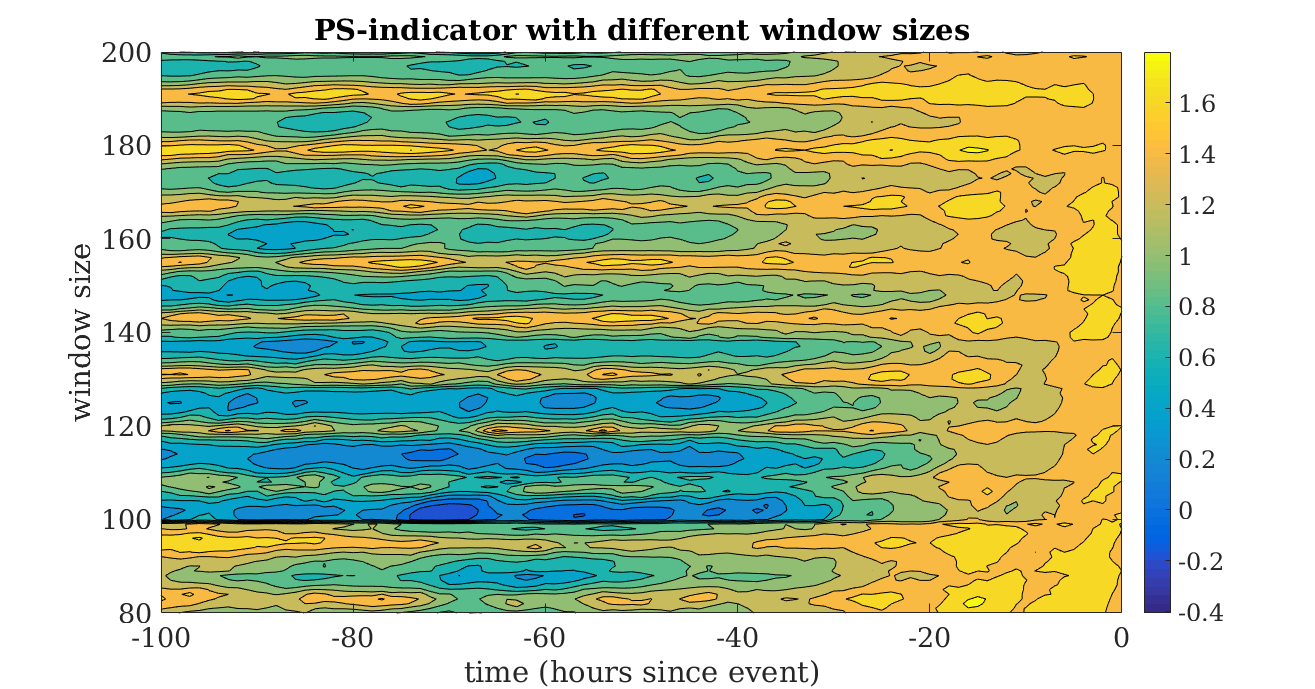
\includegraphics[width = 0.99\textwidth]{contourplot.png} \caption{ Measurement of the PS- indicator from the sea-level pressure data sets from the 14 tropical cyclones.  The measurement is repeated using a range of window sizes and the result shown as a contour plot.}
							\end{figure}
							
							
The method described provides an estimate of the changes in the PS scaling exponent in a window of 100 points. It is desirable to use a very large number of points to give an accurate estimate of the scaling exponent, less sensitive to periodic oscillations in the data and with less variability over time. However, we must compromise this since the window size must correspond to the time scale of the phenomenon under investigation; of course there is also a limit imposed by the length of the time series data. The number of points used must be a compromise with requirements:\\
\vspace{0.3cm}
\begin{enumerate}
\setlength{\itemindent}{3em}
\item the indicator variance is sufficiently small that we can see the EWS, but
\item the rise in the indicator value is large enough that we recognise it as an EWS.
\end{enumerate}
\vspace{0.3cm}
By regarding the contour plot above, we make a subjective choice as to the optimum window size to use in the context.\\
\vspace{0.8cm}
 In the figure we see that there is an increasing trend in the PS-indicator towards the end of the time series with almost all window sizes. The exceptions occur periodically where the window size is approximately $12n\pm 1$ for integer $n$. Note that the most obvious signals occur with window sizes 102, 114 and 126. Using larger values (e.g. 174) the useful variability in the indicator is smoothed out so that the trend towards the end of the series is less obvious.    			
    			
    			
    			\end{block}
    		
    		
   			
    	   
    	   
    			
   		
   			
   			\begin{block}{References}
    			        {
        
 [1] Livina, V. N., Kwasniok, F., Lohmann, G., Kantelhardt, J. W., and Lenton, T. M. (2011). Changing climate states and stability: from Pliocene to present. {\it \footnotesize Climate dynamics, 37(11-12), 2437-2453.}
        
        [2] Held, H. and Kleinen, T. (2004). Detection of climate system bifurcations by degenerate fingerprinting. {\it \footnotesize Geophys. Res. Lett. 31, L23207.}
            
        [3] Kantelhardt, J. W., Koscielny-Bunde, E., Rego, H. H., Havlin, S., and Bunde, A. (2001). Detecting long-range correlations with detrended fluctuation analysis. {\it \footnotesize Physica A: Statistical Mechanics, 295(3):441-454.}            
            
        [4]  Dakos, V., Scheffer, M., van Nes, E. H., Brovkin, V.,Petoukhov, V. and Held, H. (2008). Slowing down as an early warning signal for abrupt climate change. {\it \footnotesize Proc. Nat. Acad. Sci. USA 105, 14308-14312.}
        
        [5] Livina, V.N., Kwasniok, F., Lohmann, G., Kantelhardt, J.W. and Lenton, T.M., (2011). Changing climate states and stability: from Pliocene to present. {\it \footnotesize Climate dynamics, 37(11-12), pp.2437-2453.}
        
        [6] Lenton, T. M., Held, H., Kriegler, E., Hall, J. W., Lucht,W., Rahmstorf, S. and Schellnhuber, H. J. (2008). Tipping elements in the Earth's climate system. {\it \footnotesize Proc. Nat. Acad. Sci. USA 105, 1786-1793.}  
        
        [7] Kwasniok, F. and Lohmann, G. (2009). Deriving dynamical models from paleoclimatic records: Application to glacial millennial-scale climate variability. {\it \footnotesize Phys. Rev. E, 80(6), p.066104.}
        
        [8] Prettyman, J., Kuna, T., and Livina, V. (2018). A novel scaling indicator of early warning signals helps anticipate tropical cyclones. {\it \footnotesize EPL (Europhysics Letters), 121(1), 10002.}
            
            
            
        }
    			\end{block}
   		\end{column} 
   	
   	\end{columns}
   	
   	
   	
   	
   	
   	
   	
   	
   	
   	
    	


	 	
%\vspace{1cm}
\end{frame}


\end{document}
 
 
 
 
 
 
 
 
 
 
 
 
 
 


%%%%%%%%%%%%%%%%%%%%%%%%%%%%%%%%%%%%%%%%%%%%%%%%%%%%%%%%%%%%%%%%%%%%%%%%%%%%%%%%%%%%%%%%%%%%%%%%%%%%
%%% Local Variables: 
%%% mode: latex
%%% TeX-PDF-mode: t
